% Template per generare 

\documentclass[a4paper,11pt]{article}
\usepackage{lmodern}
\renewcommand*\familydefault{\sfdefault}
\usepackage{sfmath}
\usepackage[utf8]{inputenc}
\usepackage[T1]{fontenc}
\usepackage[italian]{babel}
\usepackage{indentfirst}
\usepackage{graphicx}
\usepackage{tikz}
\usepackage{listings}
\newcommand*\circled[1]{\tikz[baseline=(char.base)]{
		\node[shape=circle,draw,inner sep=2pt] (char) {#1};}}
\usepackage{enumitem}
% \usepackage[group-separator={\,}]{siunitx}
\usepackage[left=2cm, right=2cm, bottom=3cm]{geometry}
\frenchspacing

\newcommand{\num}[1]{#1}

% Macro varie...
\newcommand{\file}[1]{\texttt{#1}}
\renewcommand{\arraystretch}{1.3}
\newcommand{\esempio}[2]{
\noindent\begin{minipage}{\textwidth}
\begin{tabular}{|p{11cm}|p{5cm}|}
	\hline
      \textbf{\file{input (da stdin)}} & \textbf{\file{output (su stdout)}}\\
	\hline
	\tt \small #1 &
	\tt \small #2 \\
	\hline
\end{tabular}
\end{minipage}
}

% Dati del task
\newcommand{\gara}{IOI 2002}
\newcommand{\nome}{Specchio}
\newcommand{\nomebreve}{specchio}

\begin{document}
% Intestazione
\noindent{\Large \gara}
\vspace{0.5cm}

\noindent{\Huge \textbf \nome~(\texttt{\nomebreve})}

% Descrizione del task
\section*{Descrizione del problema}

Un \emph{albero} \`e formato da una \emph{radice} e da un insieme finito e ordinato (eventualmente vuoto) di \emph{figli}, che sono anch'essi alberi. Ad esempio, la Figura~1 rappresenta un albero: per convenzione, la radice viene disegnata in cima (cio\`e al contrario rispetto agli alberi veri). Come ogni albero, lo potete descrivere dicendo quanti figli ha la radice (in questo caso, quattro) e poi descrivendo uno a uno, nell'ordine da sinistra a destra, i quattro sottoalberi. In questo modo, ad esempio, l'albero in Figura~1 sarebbe identificato dalla seguente sequenza:
\[
4\,\,\,2\,\,\,0\,\,\,3\,\,\,0\,\,\,0\,\,\,1\,\,\,0\,\,\,0\,\,\,0\,\,\,0
\]	

\begin{figure}[h!]
  \centering
    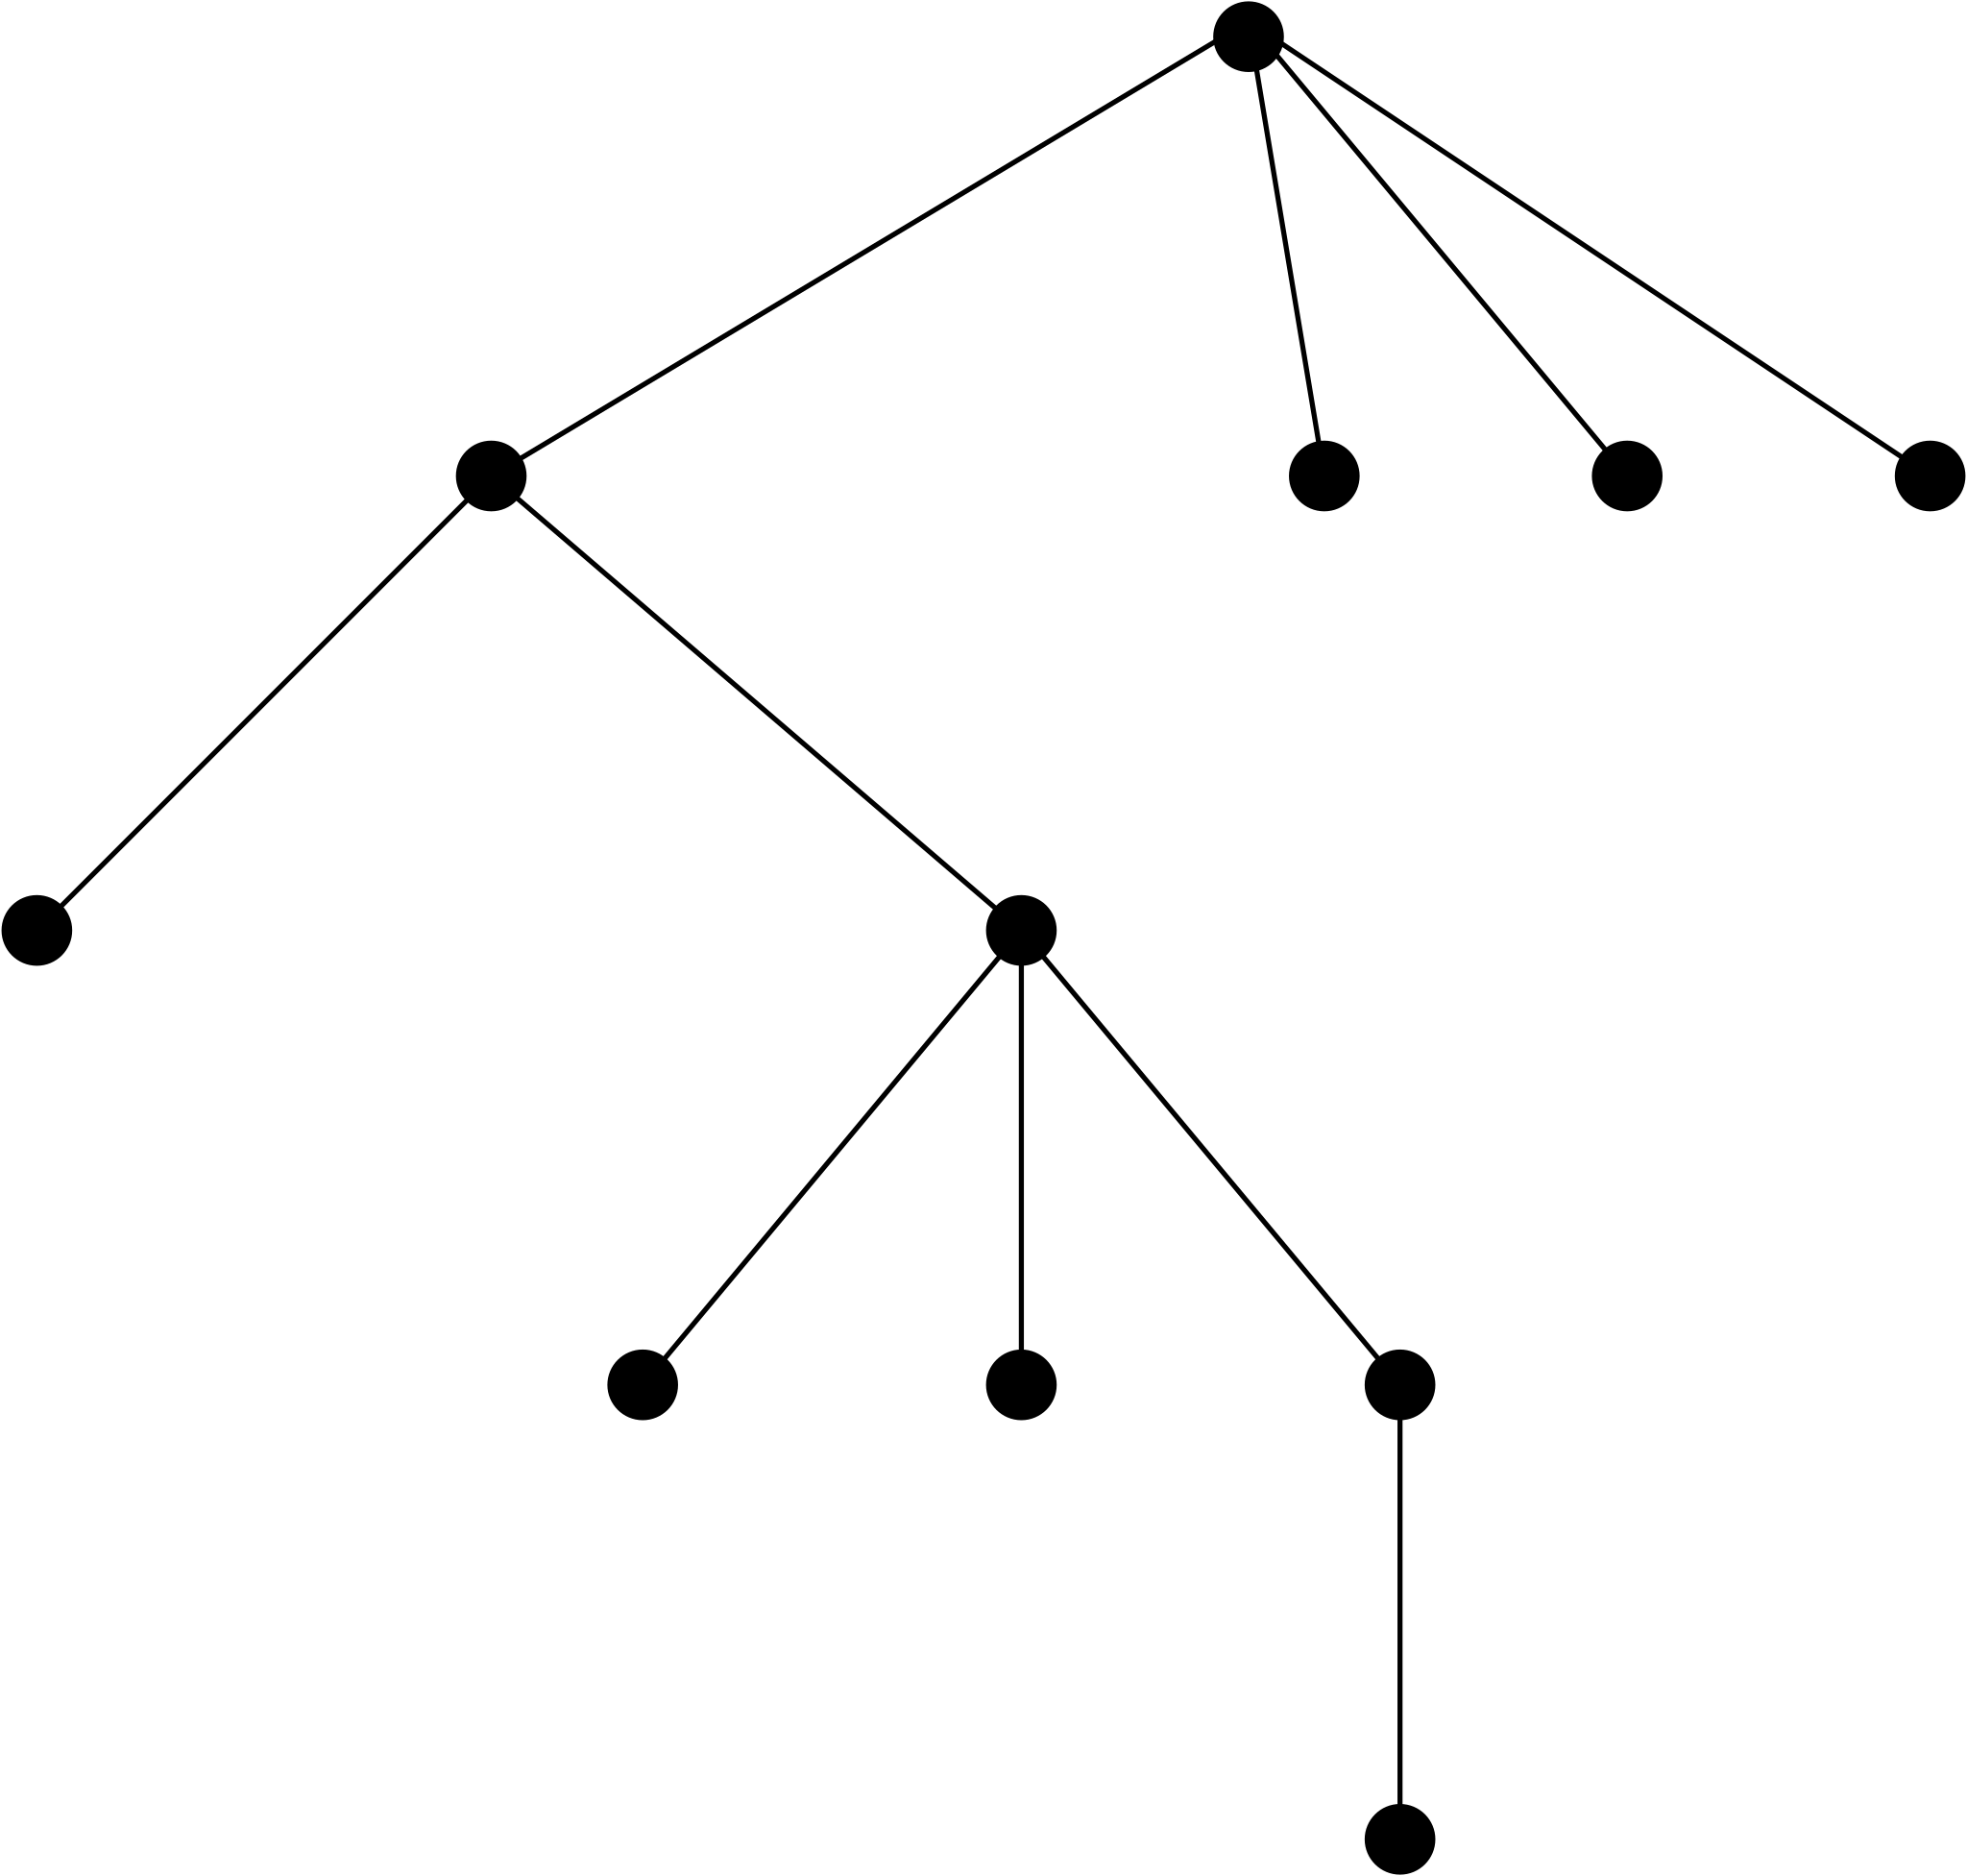
\includegraphics[scale=0.3]{figs/fig1.pdf}\\
    \caption{Un albero.}
\end{figure}

Infatti, l'albero ha quattro figli sotto la radice, per cui il primo numero \`e $4$. A questo $4$ segue poi subito la sequenza $2\,\,\,0\,\,\,3\,\,\,0\,\,\,0\,\,\,1\,\,\,0$, che \`e la descrizione del primo figlio, mentre gli ultimi tre figli sono ciascuno descritti da $0$ (dato che non hanno figli).

Supponete ora di guardare l'albero riflesso in uno specchio. L'ordine dei figli di ciascun nodo risulta invertito e l'albero di Figura~1 appare come in Figura~2.

\begin{figure}[h!]
  \centering
    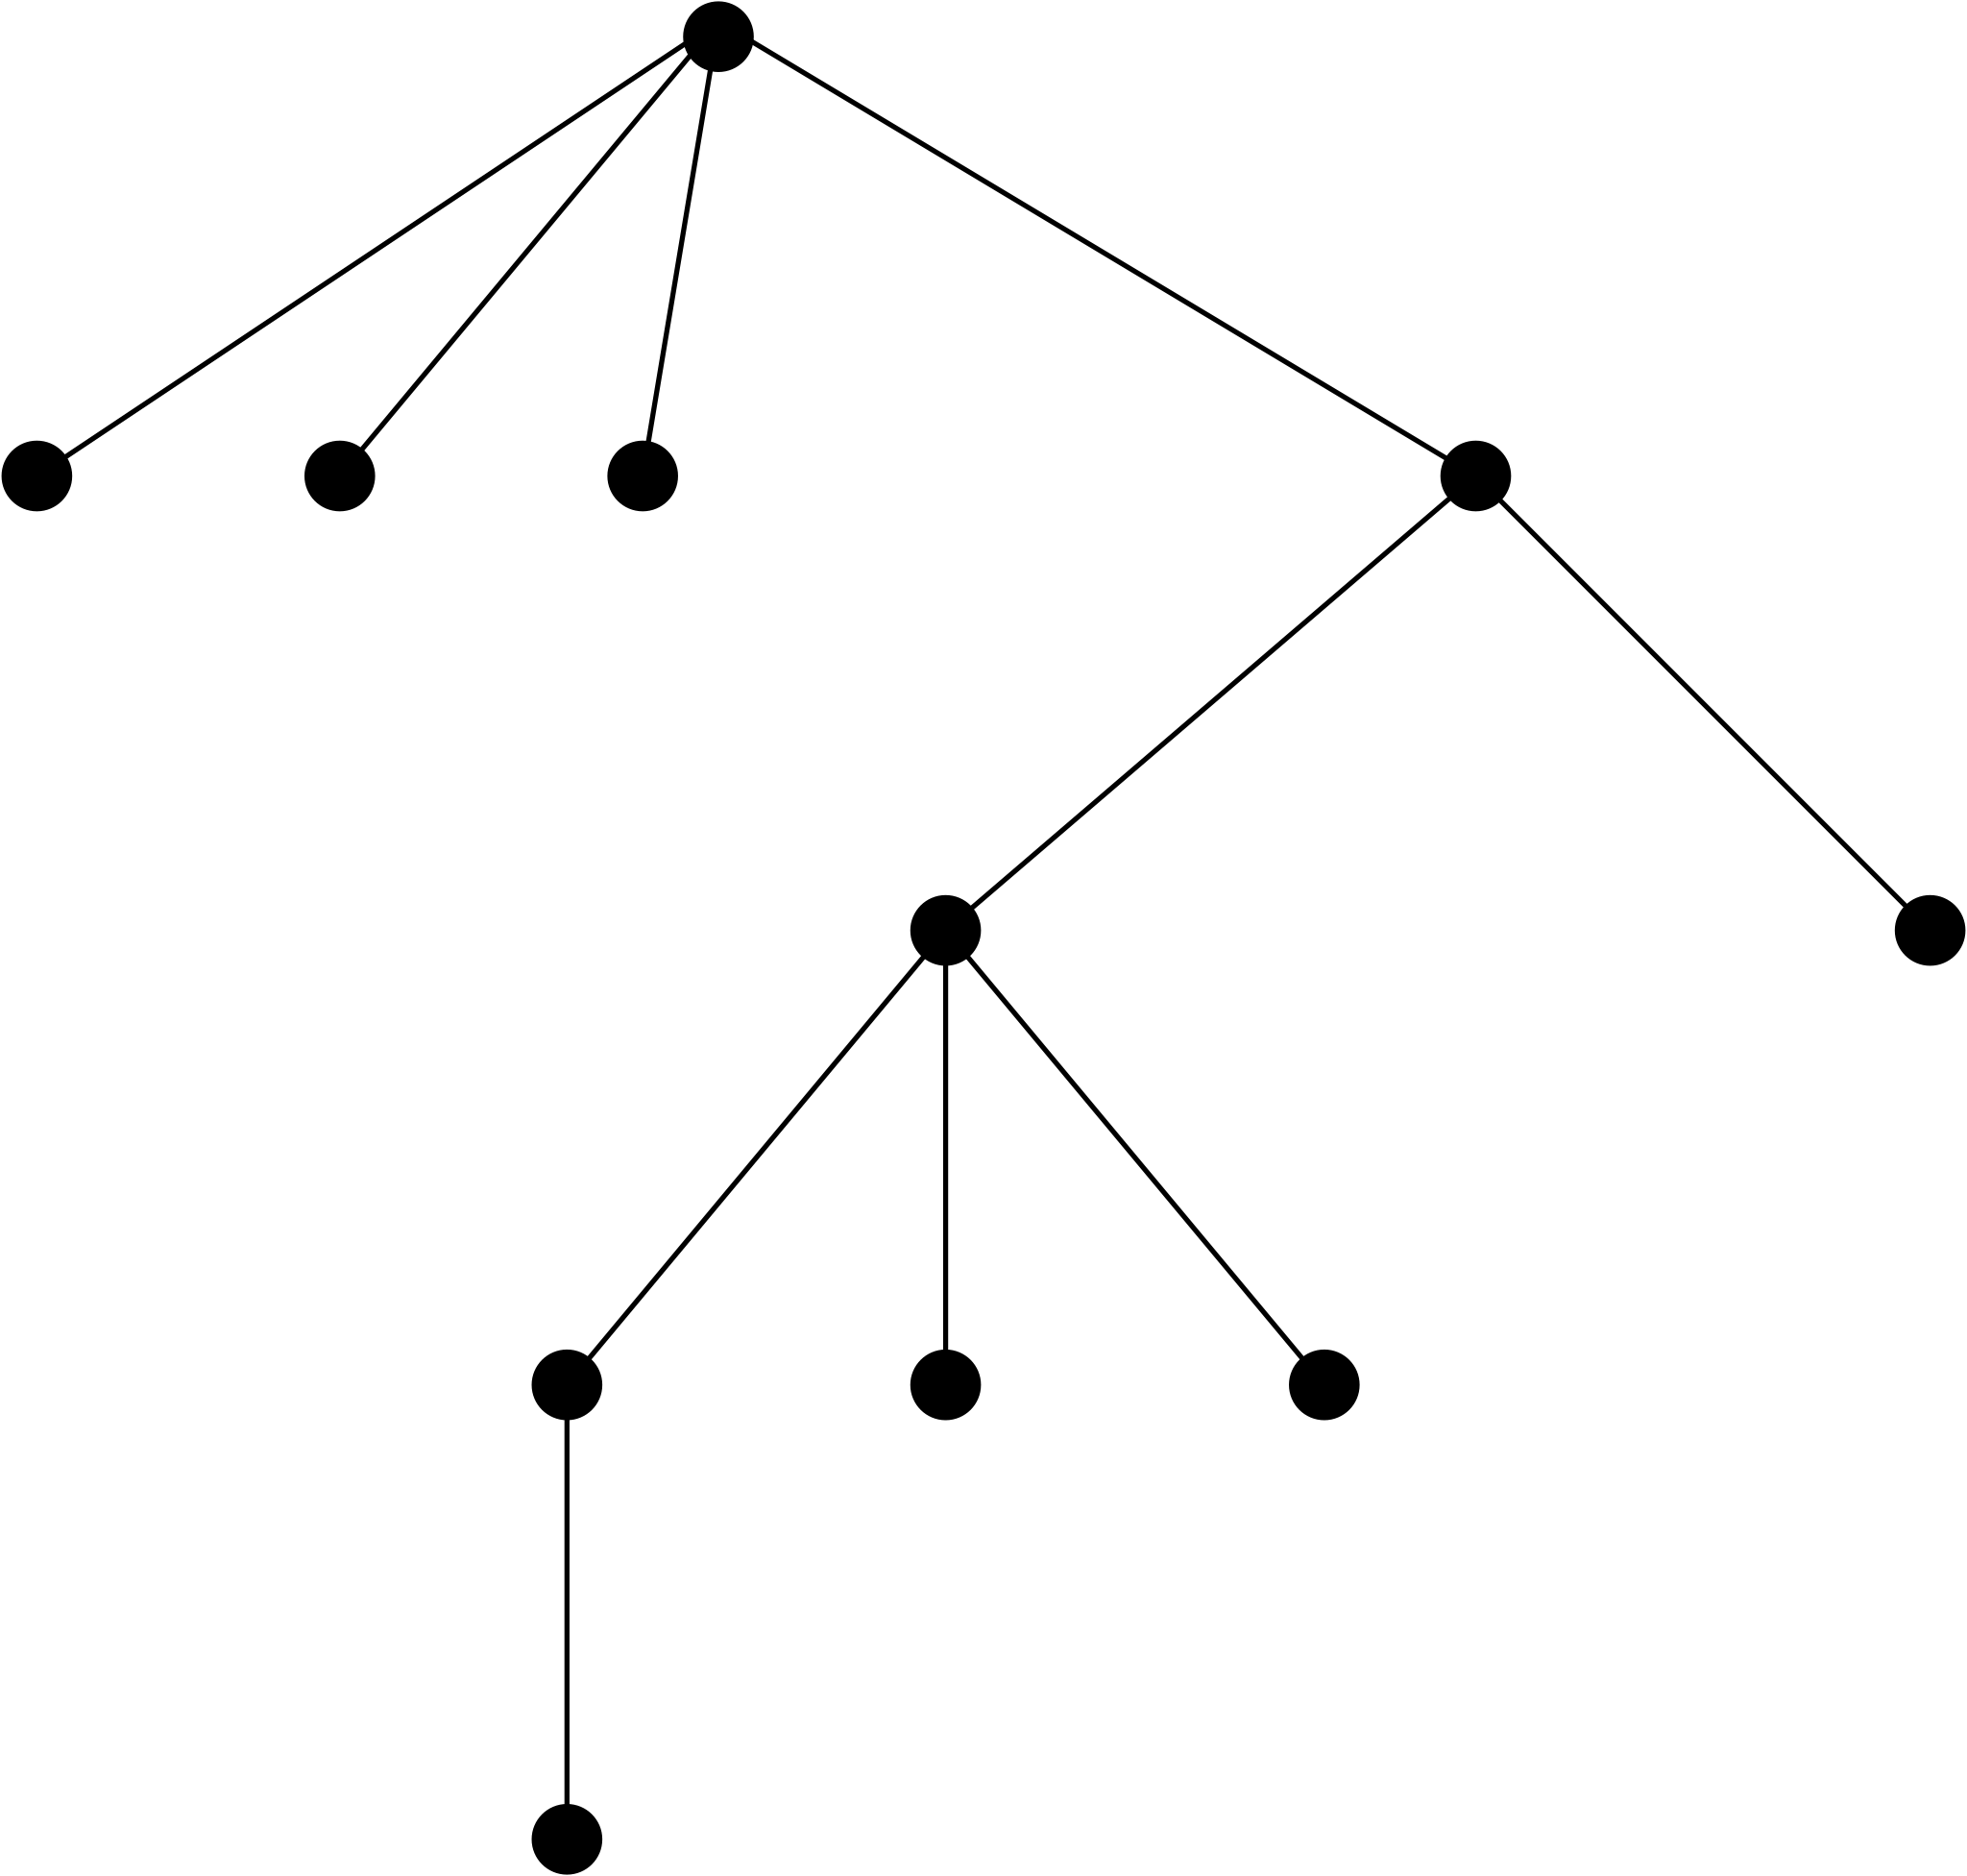
\includegraphics[scale=0.3]{figs/fig2.pdf}\\
    \caption{L'albero di Figura~1 allo specchio.}
\end{figure}

Questo nuovo albero \`e descritto dalla sequenza
\[
4\,\,\,0\,\,\,0\,\,\,0\,\,\,2\,\,\,3\,\,\,1\,\,\,0\,\,\,0\,\,\,0\,\,\,0
\]

% Input
\section*{Dati di input}

Il vostro programma legge da \verb'stdin' una sola riga contenente una sequenza di interi non negativi, separati da uno spazio. La sequenza descrive correttamente un albero: quindi il primo numero \`e il numero di figli della radice, ed \`e seguito dalle descrizioni dei figli, uno dopo l'altro, da sinistra a destra.

% Output
\section*{Dati di output}

Il vostro programma deve restituire su \verb'stdout' una sola riga, costituita da una sequenza di interi non negativi separati da uno o pi\`u spazi. Questa sequenza \`e la descrizione dell'albero dato in input, visto allo specchio.

% Esempi
\section*{Esempio di input/output}
\esempio{
4 2 0 3 0 0 1 0 0 0 0
}{
4 0 0 0 2 3 1 0 0 0 0
}

% Assunzioni
\section*{Assunzioni}
\begin{itemize}[nolistsep, noitemsep]
\item dove $N$ \`e il numero di nodi dell'albero,
      vale sempre che $1 \le N \le 1\,000\,000 $;
\item tempo limite: un secondo.
\end{itemize}

% Subtasks
\section*{Subtask}
\begin{itemize}
\item \textbf{Subtask 1 [0 punti]:} l'esempio del testo.
\item \textbf{Subtask 2 [20 punti]:} ogni nodo ha massimo due figli.
\item \textbf{Subtask 3 [20 punti]:} $N \le 100$.
\item \textbf{Subtask 4 [20 punti]:} $N \le 10\,000$.
\item \textbf{Subtask 5 [20 punti]:} $N \le 100\,000$.
\item \textbf{Subtask 6 [20 punti]:} nessuna limitazione specifica.
\end{itemize}


\end{document}
